\documentclass[11pt]{article}
\usepackage[utf8]{inputenc}

%%%%%%%%%%%%%%%%%%%%%%%%%%%%%%%%%%%%%%%%%%%%%%%%%%%%%%%%%%%%%%%%
% PACKAGES, FORMATTING, LISTING, AND OTHER GRAPHICAL ELEMENTS  %
%%%%%%%%%%%%%%%%%%%%%%%%%%%%%%%%%%%%%%%%%%%%%%%%%%%%%%%%%%%%%%%%

\usepackage{amsmath,amssymb}
\usepackage[T1]{fontenc} % font encoding
\usepackage{graphicx} % for figures
\usepackage{float} % for figures
\usepackage{indentfirst} % indent first paragraph of section
\usepackage{soul,xcolor} % for colors
\usepackage{xkcdcolors} % colors from XKCD color survey
\usepackage{mathtools} % for boxed equations within \align
\usepackage{sectsty} % adjust section headers
\usepackage{fancyhdr} % page headers
\usepackage{titling} % reference title,author,date (in fancyhdr page header)
\usepackage{breqn} % automatically line wrap long Eqs.
\usepackage{pdfpages} % for \includepdf
\usepackage{pdflscape} % landscape 
\usepackage{mdframed} % for framed environment
\usepackage{listings} % for code blocks
\usepackage{inconsolata} % better monospace font
\usepackage{matlab-prettifier} % Better MATLAB listing highlighting
\usepackage[letterpaper, total={6.5in, 9in}]{geometry} % set paper and margin size
\usepackage{empheq} % multiline boxed equations, etc.
\usepackage{hyperref}
\usepackage{dsfont}	% gives you \mathds{} font
% \usepackage{enumerate} % custom enumerate numbering (or lettering in this case)
\usepackage[shortlabels]{enumitem} % more enumerate options
\usepackage{svg} % use inkscape to import svgs
\usepackage{bm} % bold symbols
\usepackage[parfill]{parskip} % replace indentation with paragraph spacing
\usepackage{dsfont} % gives you \mathds{} font

% hyperbolic trig inverse functions
\DeclareMathOperator{\sech}{sech}
\DeclareMathOperator{\csch}{csch}
\DeclareMathOperator{\arcsec}{arcsec}
\DeclareMathOperator{\arccot}{arcCot}
\DeclareMathOperator{\arccsc}{arcCsc}
\DeclareMathOperator{\arccosh}{arcCosh}
\DeclareMathOperator{\arcsinh}{arcsinh}
\DeclareMathOperator{\arctanh}{arctanh}
\DeclareMathOperator{\arcsech}{arcsech}
\DeclareMathOperator{\arccsch}{arcCsch}
\DeclareMathOperator{\arccoth}{arcCoth} 

% add page headers
\pagestyle{fancy}
\fancyhf{}
\fancyhead[LE,LO]{\thetitle}
\fancyhead[RE,RO]{\theauthor}
\fancyfoot[CE,CO]{\thepage}

% adjust section header font size
\sectionfont{\fontsize{20}{15}\selectfont}
\subsectionfont{\fontsize{14}{15}\selectfont}

% vertical table spacing
\renewcommand{\arraystretch}{1.5}

% right-side cases
% \newenvironment{rcases}
%     {\left.\begin{aligned}}
%     {\end{aligned}\right\rbrace}

% Multi-line \fbox
\newcommand\multilineBox[1]{
\noindent
\fbox{
	\parbox{0.97\linewidth}
		{#1}
	}
}

% number just one equation in an un-numbered align* environment
\newcommand\numberthis{\addtocounter{equation}{1}\tag{\theequation}}

%%%%%%%%%%%%%%%%%%%%%%%%%%%%%%%%%%%%%%%%%%%%%%%%%%%%%%%%%%%%%%%%

% set listings font to inconsolata
\DeclareFixedFont{\ttb}{T1}{txtt}{bx}{n}{9} % for bold
\DeclareFixedFont{\ttm}{T1}{txtt}{m}{n}{9}  % for normal

% general listings environment
\lstnewenvironment{code}
{\lstset{
    frame=single,
    % backgroundcolor=\color{xkcdPale},
    basicstyle=\fontfamily{pcr}\selectfont\tiny
    }}
{}

% MATLAB listings environment
\lstnewenvironment{MATLAB}
{\lstset{
    style=Matlab-editor,
    frame=single,
    % backgroundcolor=\color{xkcdPale},
    basicstyle=\fontfamily{pcr}\selectfont\tiny
    }}
{}

% Python style for listings
\newcommand\pythonstyle{\lstset{
    language=Python,
    basicstyle=\ttm,
    morekeywords={self},              % Add keywords here
    keywordstyle=\ttb\color{xkcdGreen},
    morekeywords=[2]{
        array,
        pi,
        zeros,
        max,
        sin,
        cos,
        linspace,
        size,
        plot,
        xlabel,
        title,
        legend,
        show,
        concatenate,
        logspace,
        exp,
        ylabel,
        savefig,
        grid,
        figure,
        axes
    },
    keywordstyle = [2]{\color{xkcdBrightBlue}},
    emph={__init__},                  % Custom highlighting
    emphstyle=\ttb\color{xkcdRed},    % Custom highlighting style
    stringstyle=\color{xkcdGreen},
    backgroundcolor=\color{xkcdPale},
    numberstyle=\color{xkcdGrey},
}}

% Python listings environment
\lstnewenvironment{python}[1][]
{\pythonstyle \lstset{#1}}
{}

% Python listings for external files
\newcommand\pythonexternal[2][]
{{\pythonstyle \lstinputlisting[#1]{#2}}}

% Python listings inline
\newcommand\pythoninline[1]{{\pythonstyle \lstinline!#1!}}


%%%%%%%%%%%%%%%%%%%%%%%%%%%%%%%%%%%%%%%%%%%%%%%%%%%%%%%%%%%%%%%%
% MATHEMATICAL SHORTCUTS                                       %
%%%%%%%%%%%%%%%%%%%%%%%%%%%%%%%%%%%%%%%%%%%%%%%%%%%%%%%%%%%%%%%%

% real and imaginary components
\renewcommand{\Re}{\operatorname{Re}}
\renewcommand{\Im}{\operatorname{Im}}

% Fourier transforms
\newcommand\fourier[1]{\frac{1}{\sqrt{2\pi}} \int_{-\infty}^\infty #1 e^{-i\omega x} \textrm{d}x}
\newcommand\inverseFourier[1]{\frac{1}{\sqrt{2\pi}} \int_{-\infty}^\infty #1 e^{i\omega x} \textrm{d}\omega}

% derivatives
\newcommand{\ppf}[2]{\frac{\partial #1}{\partial #2}}
\newcommand{\pppf}[3]{\frac{\partial^2 #1}{\partial #2 \partial #3}}
\newcommand{\ddf}[2]{\frac{\text{d} #1}{\text{d} #2}}
\newcommand{\DDf}[2]{\frac{\text{D} #1}{\text{D} #2}}

% norms
\newcommand\norm[1]{\lVert#1\rVert}

% statistical operators
\newcommand{\prob}{\operatorname{P}}
\newcommand{\expectation}{\operatorname{E}}
\newcommand{\variance}{\operatorname{Var}}
\newcommand{\stddev}{\operatorname{SD}}

% statistical distributions
\newcommand{\bernoulli}{\operatorname{Bernoulli}}
\newcommand{\binomial}{\operatorname{Binomial}}
\newcommand{\poisson}{\operatorname{Poisson}}
\newcommand{\normal}{\operatorname{Normal}}

%%%%%%%%%%%%%%%%%%%%%%%%%%%%%%%%%%%%%%%%%%%%%%%%%%%%%%%%%%%%%%%%
% COMMONLY USED COPYPASTAS
%%%%%%%%%%%%%%%%%%%%%%%%%%%%%%%%%%%%%%%%%%%%%%%%%%%%%%%%%%%%%%%%

% CODE BLOCK

% \begin{MATLAB}[caption={MATLAB script},label={code:p1}]
% for i = 1:n
%     disp('string')
% end
% \end{MATLAB}
% Code block \ref{code:p1}



% MULTIPLE EQUATIONS BOXED

% \begin{empheq}[box=\fbox]{align}
% \end{empheq}



% ENUMERTATE WITH a) instead of 1.

% \begin{enumerate}[label=\alph*)]
% \end{enumerate}
% 'Problem' sections
% \renewcommand{\thesection}{Part \arabic{section}}
\renewcommand{\thesubsection}{\arabic{section}.\alph{subsection}}
% \renewcommand{\thesubsection}{\arabic{subsection}}

\title{ENGR 510 ODE Homework}
\author{Anthony Su}
\date{October 18, 2024}

\begin{document}
\thispagestyle{plain}
\maketitle


%%%%%%%%%%%%%%%%%%%%%%%%%%%%%%%%%%%%%%%%%%%%%%%%%%%%%%%%%%%%%%%%
% EXERCISE 1
%%%%%%%%%%%%%%%%%%%%%%%%%%%%%%%%%%%%%%%%%%%%%%%%%%%%%%%%%%%%%%%%
\section{}
\begin{align*}
    \dot{x} = \lambda x, \quad x(0) = 1
\end{align*}


\subsection{}  % 1.a -------------------------------------------
General solution by separation of variables:
\begin{align*}
    \ddf{x}{t} &= \lambda x \\
    \frac{\text{d}x}{x} &= \lambda \text{d}t \\
    \ln(x) &= \lambda t + C \\
    x(t) &= e^{\lambda t + C} \\
    x(t) &= k e^{\lambda t}
\end{align*}
Applying the initial condition:
\begin{align*}
    x(0) &= k e^{\lambda \cdot 0} \\
    1 &= k
\end{align*}
Therefore, the particular solution is:
\begin{align*}
    \Aboxed{
    x(t) = e^{\lambda t}
    }
\end{align*}


\subsection{}  % 1.b -------------------------------------------
\begin{figure}[H]
    \centering
    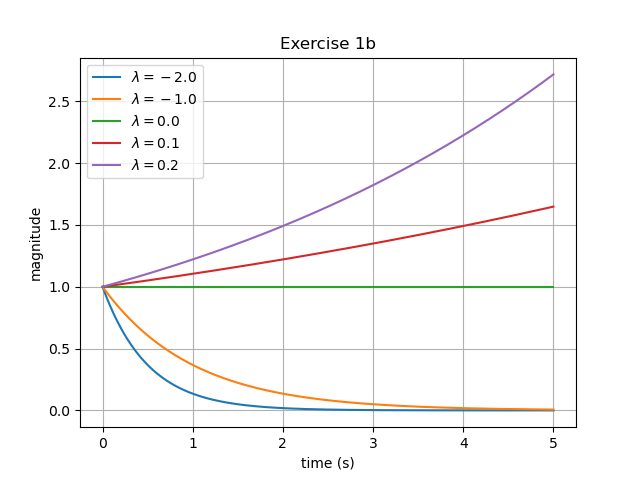
\includegraphics[width=0.8\textwidth]{1b_fig1.png}
    \caption{Solution to $\dot{x}=\lambda x$ for various values of $\lambda$}
    \label{fig_1b1}
\end{figure}

\subsection{}  % 1.c -------------------------------------------
Positive values of $\lambda$ diverge to infinity, negative values of $\lambda$ converge to zero, and $\lambda=0$ remains constant.


%%%%%%%%%%%%%%%%%%%%%%%%%%%%%%%%%%%%%%%%%%%%%%%%%%%%%%%%%%%%%%%%
% EXERCISE 2
%%%%%%%%%%%%%%%%%%%%%%%%%%%%%%%%%%%%%%%%%%%%%%%%%%%%%%%%%%%%%%%%
\section{}
\begin{align*}
    \ddot{x} - \lambda x &= 0
\end{align*}

\subsection{}  % 2.a -------------------------------------------
Guess $x(t) = e^{l t}$:
\begin{align*}
    x(t) &= e^{l t} \\
    \ddf{x}{t} &= l e^{l t} \\
    \ddf{^2 x}{t^2} &= l^2 e^{l t}
\end{align*}
Generate characteristic polynomial by substitution into the ODE: % assuming that constant in the equation is same as lambda
\begin{align*}
    l^2 e^{l t} - \lambda e^{l t} &= 0 \\
    e^{\lambda t} \left( l^2 - \lambda \right) &= 0 \\
    l^2 - \lambda &= 0
\end{align*}
Solutions to the characteristic polynomial are $l=\pm\sqrt{\lambda}$. The general solution is the linear combination of the particular solutions:
\begin{align*}
    x(t) &= C_1 e^{\sqrt{\lambda} t} + C_2 e^{-\sqrt{\lambda} t}
\end{align*}
The first derivative is:
\begin{align*}
    \dot{x}(t) &= C_1 \sqrt{\lambda} e^{\sqrt{\lambda} t} - C_2 \sqrt{\lambda} e^{-\sqrt{\lambda} t}
\end{align*}
Applying initial conditions given by $x(0)$ and $\dot{x}(0)$:
\begin{align*}
    x(0) &= C_1 + C_2 \\
    \dot{x}(0) &= C_1 \sqrt{\lambda} - C_2 \sqrt{\lambda}
\end{align*}
Solving the system of equations yields $C_1 = \frac{1}{2} \left( x(0) + \frac{\dot{x}(0)}{\sqrt{\lambda}} \right)$ and $C_2 = \frac{1}{2} \left( x(0) - \frac{\dot{x}(0)}{\sqrt{\lambda}} \right)$. Thus, the general solution to the ODE is
\begin{align*}
    \Aboxed{
    x(t) &= \frac{1}{2} \left( x(0) + \frac{\dot{x}(0)}{\sqrt{\lambda}} \right) e^{\sqrt{\lambda} t} + \frac{1}{2} \left( x(0) - \frac{\dot{x}(0)}{\sqrt{\lambda}} \right) e^{-\sqrt{\lambda} t}
    }
\end{align*}

\subsection{}  % 2.b -------------------------------------------
When $\lambda > 0$, all quantities are real and the solution diverges due to the positive exponent in the first term. When $\lambda < 0$, the exponents are purely imaginary so oscillatory behavior without damping ensues.

\subsection{}  % 2.c -------------------------------------------
\begin{figure}[H]
    \centering
    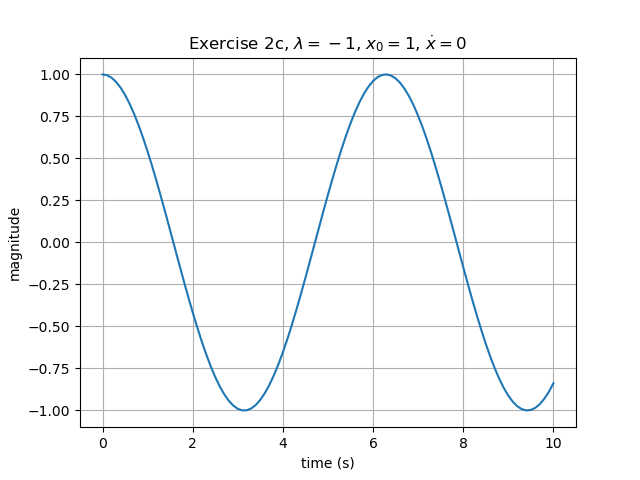
\includegraphics[width=0.8\textwidth]{2c_fig1.png}
    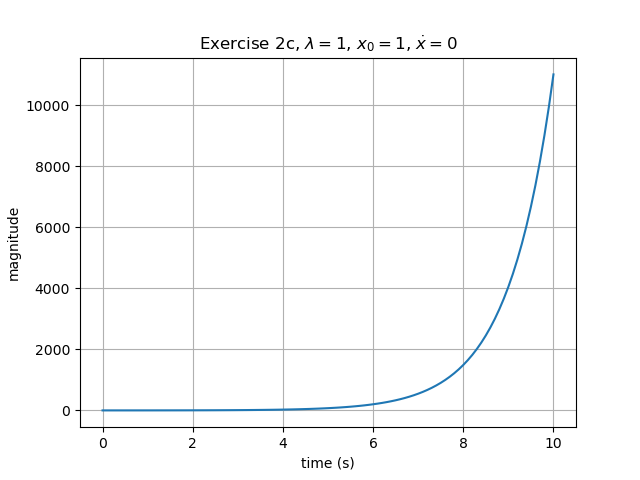
\includegraphics[width=0.8\textwidth]{2c_fig2.png}
    \caption{Solution to $\ddot{x}=\lambda x$ for various values of $\lambda$}
    \label{fig_2c1}
\end{figure}


%%%%%%%%%%%%%%%%%%%%%%%%%%%%%%%%%%%%%%%%%%%%%%%%%%%%%%%%%%%%%%%%
% EXERCISE 3
%%%%%%%%%%%%%%%%%%%%%%%%%%%%%%%%%%%%%%%%%%%%%%%%%%%%%%%%%%%%%%%%
\section{}

\subsection{}  % 3.a -------------------------------------------
The eigenvalues $(-1, -3)$ are negative real numbers, so the exponential result converges without oscillation.

\subsection{}  % 3.b -------------------------------------------
The eigenvalues $(0+2i, 0-2i)$ are purely imaginary which results a system that is purely oscillatory with no damping.

\subsection{}  % 3.c -------------------------------------------
The eigenvalues (-2, 4) have at least one with a positive real component, so the exponential solution diverges.

\end{document}